\documentclass[a4paper]{report}
\usepackage[margin=1cm]{geometry}
\usepackage{tikz,tikz-dimline}
\usetikzlibrary{patterns}
\pgfplotsset{compat=1.18} 

\begin{document}
\pagestyle{empty}

\begin{tikzpicture}[overlay,shift={(0,-28)}]
\draw [line width=1mm](0,0) rectangle (19,29);
\draw [line width=0.5mm] (0,0) rectangle (19,1);
\draw (0,0.5) node [right]{DIRECCIÓN:\textbf{SAN ANDRES 129} OBRA:\textbf{AMPLIACIÓN} };
\end{tikzpicture}

\begin{center}
\scalebox{1.7}{
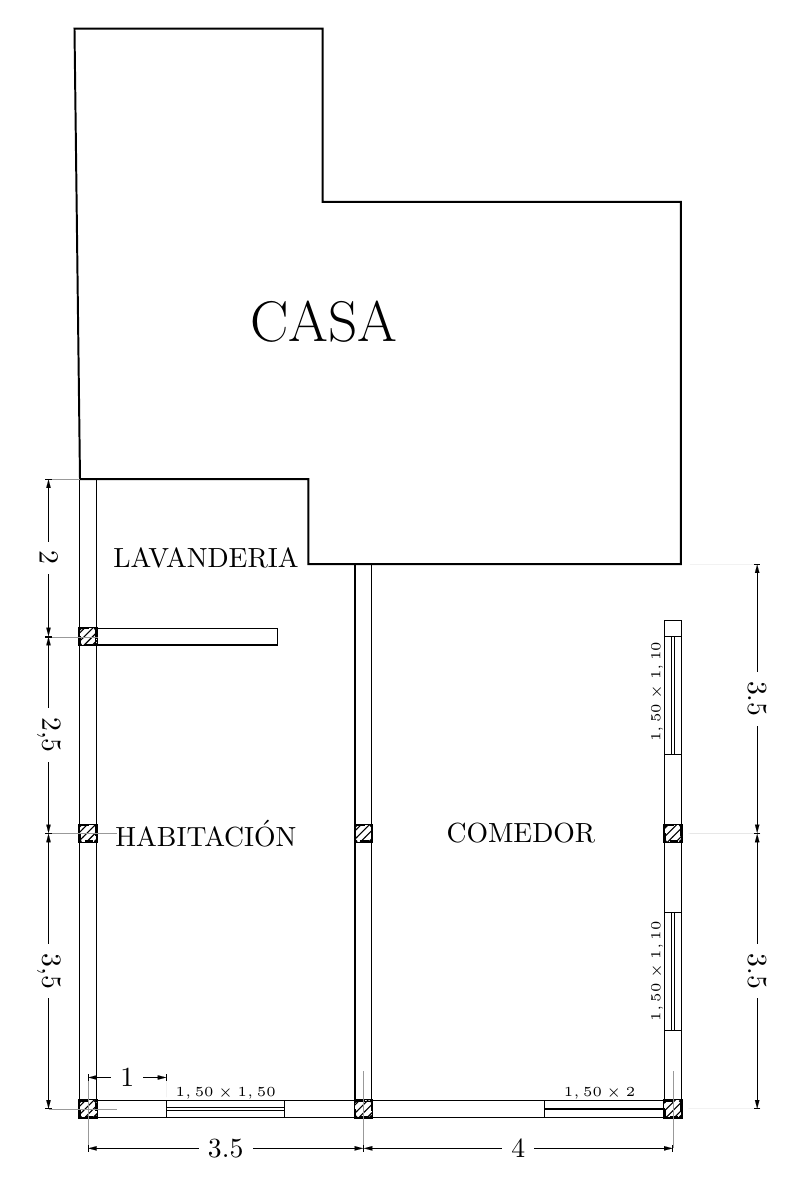
\begin{tikzpicture}
%----------zapata---------
\tikzset{zapata/.style={
rectangle,
draw,
pattern=north east lines,
minimum size=2mm,
path picture={%
    \draw[fill=black] (1mm,1mm) circle (0.15mm);
    \draw[fill=black] (-1mm,-1mm) circle (0.15mm);
    \draw[fill=black] (1mm,-1mm) circle (0.15mm);
    \draw[fill=black] (-1mm,1mm) circle (0.15mm);
    \draw [dashed,line width=0.2mm] (-1mm,-1mm)rectangle(1mm,1mm);
    }}};


\draw [cap=rect,double,double distance=2mm](0,-2.1)-- (0,-10)--(7.43,-10)--(7.43,-3.9);
\draw [cap=rect,double,double distance=2mm](3.5,-3.18)--(3.5,-9.8);
\draw [cap=rect,double,double distance=2mm](0.2,-4)--(3.5-1.2,-4);

\draw (3,0) node {\huge CASA};
\draw (1.5,-3) node {LAVANDERIA};
\draw (1.5,-6.5) node {HABITACIÓN};
\draw (5.5,-6.5) node {COMEDOR};

%------------ zapatas---------------
\node [zapata,shift=({0,-4})]{};
\node [zapata,shift=({0,-6.5})]{};
\node [zapata,shift=({0,-10})]{};
\node [zapata,shift=({3.5,-10})]{};
\node [zapata,shift=({7.43,-10})]{};
\node [zapata,shift=({3.5,-6.5})]{};
\node [zapata,shift=({7.43,-6.5})]{};

% -----------cotas----------------

\dimline[extension start length=-0.25, extension end length=-0.25]{(-0.5,-2)}{(-0.5,-4)}{2};
\dimline[extension start length=-0.25, extension end length=-0.25]{(-0.5,-4)}{(-0.5,-6.5)}{2,5};
\dimline[extension start length=-0.25, extension end length=-0.25]{(-0.5,-6.5)}{(-0.5,-10)}{3,5};
\dimline[extension start length=0.25, extension end length=0.25]{(8.5,-3.08)}{(8.5,-6.5)}{3.5};
\dimline[extension start length=0.25, extension end length=0.25]{(8.5,-6.5)}{(8.5,-10)}{3.5};
\dimline[extension start length=-0.25, extension end length=-0.25]{(0,-10.5)}{(3.5,-10.5)}{3.5};
\dimline[extension start length=-0.25, extension end length=-0.25]{(3.5,-10.5)}{(7.43,-10.5)}{4};

\draw [line width=0.25mm](-0.1,-2)--(2.8,-2)--(2.8,-2)--(2.8,-3.08)-- (2.8,-3.08)--(7.53,-3.08)--(7.53,1.52)--(2.98,1.52)--(2.98,3.72)--(-0.17,3.72)--(-0.10,-2);

%puerta corrediza comedor
\draw (7.33,-10)--(5.8,-10);
\draw (5.8,-10.1)--(5.8,-9.9);
\draw (5.8,-10.1)--(5.8,-9.9);
\draw (6.5,-10) node [above]{\tiny $1,50\times2$};

%ventana habitación.
\draw (1,-10.1)--(1,-9.9);
\draw [double](1,-10)--(2.5,-10);
\draw (2.5,-10.1)--(2.5,-9.9);
\draw (1.75,-10) node [above]{\tiny $1,50\times1,50$};
\dimline[extension start length=0.25, extension end length=0.25]{(0,-9.6)}{(1,-9.6)}{1};

% ventanas comedor
% ventana lejana
\draw [double](7.43,-9)--(7.43,-7.5);
\draw (7.33,-9)--(7.53,-9);
\draw (7.33,-7.5)--(7.53,-7.5);
\draw (7.23,-8.25) node[rotate=90] {\tiny $1,50\times1,10$};

% ventana cercana
\draw [double](7.43,-5.5)--(7.43,-4.0);
\draw (7.33,-5.5)--(7.53,-5.5);
\draw (7.33,-4)--(7.53,-4);
\draw (7.23,-4.7) node[rotate=90] {\tiny $1,50\times1,10$};
\end{tikzpicture}
}
\end{center}


\end{document}